\documentclass[a4paper,12pt]{article}
\usepackage{fullpage}  % leaves 1 inch margins all round
\usepackage{iftex}
\ifPDFTeX
  \usepackage[T1]{fontenc} % modern encoding (more characters available)
  \usepackage{mathptmx} % times in text and mathematics
  \usepackage[scaled]{helvet} % helvetica for sanserif, scaled 95% by default
  \usepackage{courier}  % for typewriter text
\else
  \usepackage{fontspec}
  \usepackage{unicode-math}
  \setmainfont{Times New Roman}
  \setsansfont{Arial}
  \setmonofont{Consolas}
  \setmathfont{Cambria Math}
\fi
\usepackage{textcomp} % lots of useful symbols
\usepackage{graphicx}  % inclusion of graphics files
\usepackage{amsmath}
\usepackage{cite}


\begin{document}

\title{How to write a technical project report}
\author{School of Engineering, University of Glasgow}
\date{\today}
 
\maketitle

\begin{abstract}
All reports start with an \emph{abstract}, which contains a summary of the project: its aim, what was done and what was achieved. This document describes the requirements for a project report in the department and gives advice on how to get better marks. It is structured to match a project report as far as possible.
\end{abstract}

%\tableofcontents

\section{Introduction}

\emph{Whew -- I've finished the work, now I only have to write the report.} Sound familar? Many students put off writing until too late and don't leave enough time to make a good job of the report. This is a serious mistake because the report typically accounts for a large fraction of the assessment. Start early -- most people find report-writing difficult. Think about the report throughout your project, keep track of references and collect material to illustrate the report.

\subsection{Mechanical aspects}

The length of the body of the report will be specified in the instructions for the project. Extra material may be provided in appendices but this material should be for reference only: you cannot assume that the reader will study it. In other words, do not put vital points in an appendix.

You will probably think that the report is too short but this is deliberate. Most reports are submitted to busy managers, who do not have time to read lengthy documents. It is important to learn how to pick out the vital points and write a concise report with maximum impact.

Reports should be word-processed and firmly bound. Use A4 paper and a clear typeface such as 12-point Times, number the pages and leave margins of at least 25\,mm all round. Follow this layout (this document breaks some of the rules to keep it compact).
\begin{itemize}
\item
The front cover should show the title of the project with your name(s) and matriculation number(s) and the name of your supervisor(s).
\item
Put the abstract on the next page. It should be about 100--250 words and gives a brief summary of the report including the background and aims of the project, the principal results and conclusions.
\item
The next page should show the table of contents. 
\item
The body of the report should be divided into numbered sections, each starting on a new page. Figures (diagrams, plots or photographs) and tables need captions and should be numbered.
\end{itemize}

\subsection{What goes into the introduction?}

Explain the background to the project and the reasons why your particular piece of work was considered worthwhile. This leads to the \textbf{aims} of the project: what you are trying to achieve. Be specific.


\section{Body of the report}

\subsection{Experimental protocol and basic settings}

This study includes two stages of experiments. The first stage covers the early exploratory experiments and was used to establish the initial baseline and examine the effect of input enhancement and loss design on segmentation performance. The second stage covers the later main experiments and was conducted on the DRIVE dataset \cite{staal2004drive} under a unified five-fold cross-validation setting to test the proposed structural modifications. Because the two stages differ in data sources, input form, data splitting, and evaluation metrics, they are described separately.

The early exploratory stage includes the first three experiments. This stage used multi-source data to train the initial segmentation model and to examine the effect of input enhancement and loss design. The later main stage starts from Experiment 4. Experiment 4 established the baseline setting on DRIVE. Experiment 5 and all subsequent structural variants were evaluated with the same dataset, preprocessing pipeline, and five-fold split, which ensured a fair comparison.

\subsubsection{Datasets and data organization}

During the early exploratory stage, the training data came from several public retinal vessel segmentation datasets, including STARE \cite{hoover2000locating}, CHASE\_DB1 \cite{fraz2012ensemble}, and HRF \cite{budai2013robust}. This stage used multi-source training samples to build the initial model and to examine its performance on the DRIVE target domain. The first three experiments did not use a new data split. Instead, they followed the existing training and validation lists so that the experimental setting remained consistent with the senior student's work and the results could be compared directly under the same data conditions. According to the existing split files, the training and validation sets contained 801 and 90 samples, respectively.

For the input format in the early stage, each color fundus image was converted to the NIfTI format used by nnU-Net and then split into three separate channels, red, green, and blue. These channels were used as model inputs. This design preserved the spectral information in the original images and allowed the model to learn vessel features from different color channels. It also provided the basis for later analysis of green-channel information and contrast enhancement.

The later main experiments used only the DRIVE dataset and followed a unified data organization scheme. In this stage, the input was no longer a three-channel color image. Instead, each image was processed with grayscale conversion, normalization, contrast-limited adaptive histogram equalization, and gamma correction, and then converted to a single-channel NIfTI file. This pipeline follows the preprocessing setting used in PA-Net \cite{luo2025panet} and was used to improve the visibility of thin vessels and low-contrast regions while reducing unrelated color information.

The later protocol was established from Experiment 4 onward. Experiment 4 defined the baseline setting on DRIVE. Experiment 5 and all subsequent structural variants used the same data organization, preprocessing pipeline, and five-fold split. As a result, performance differences among these models can be attributed mainly to changes in network structure, loss design, or post-processing rather than to differences in data splitting.

\subsubsection{Implementation details and evaluation metrics}

All experiments were implemented within the nnU-Net v2 framework \cite{isensee2021nnunet}. To keep the comparisons interpretable, experiments within the same stage used the same training workflow. Unless otherwise stated, differences between experiments were limited to input preprocessing, network structure, loss function, or post-processing. The later experiments were driven mainly by changes to the U-Net backbone inside nnU-Net and to the way features were exchanged across stages, while only a small number of experiments modified loss settings or trainer-level training strategies. The early exploratory stage used a fixed split to test the feasibility of different designs. The later main stage used the 2D nnU-Net configuration on DRIVE with five-fold cross-validation to evaluate the proposed modifications.

In the early stage, the baseline model used the standard nnU-Net trainer and was trained for 150 epochs. The first three experiments corresponded to the baseline with raw input, the input-enhanced version with CLAHE, and the version that combined Dice loss with Focal Loss on top of the enhanced input. The evaluation script in this stage reported IoU for the vessel class, mIoU, Recall, Precision, Accuracy, mPA, and F1-score. The early-stage results were therefore reported with this metric set.

In the later main stage, all models were trained with the 2D nnU-Net v2 configuration. The input patch size was \(512 \times 512\), the batch size was 2, and the number of training epochs was 100. The optimizer was SGD with an initial learning rate of 0.001 and a Poly learning rate schedule. Unless otherwise stated, all models used the same data split and training plan. Experiment 4 established the baseline for this stage, and Experiment 5 together with all later variants was compared under this shared setting.

For evaluation, the later main stage did not rely on the result from a single fold. Instead, the outputs from all five folds were aggregated before the final metrics were computed. Each fold produced predictions for its validation set, and the final evaluation was carried out on the complete cross-validation output. This reduced the variation introduced by a single split and improved consistency across model comparisons.

The later main stage reported Sensitivity (SE), Specificity (SP), Accuracy (ACC), AUC, Precision (PR), and F1-score. SE measured the detection of thin vessels and weak responses. SP and PR reflected the control of false positives. ACC described overall pixel-level accuracy, and F1-score gave a combined measure of segmentation performance. Because probability maps were not saved in the current experiments, the reported AUC was computed as an approximation from binary predictions.

\subsection{Baseline and early explorations}

This study started from the early baseline experiments and the associated explorations of input enhancement and loss design. The first three valid experiments did not use a new data split. Instead, they followed the existing training and validation lists so that the setting remained consistent with the senior student's work and the results could be compared directly under the same data conditions. All three experiments used DRIVE as the test dataset and were evaluated with the same early-stage metric set.

The first experiment used the standard nnU-Net baseline \cite{isensee2021nnunet} and established the initial performance reference. The results showed that the model already provided stable overall segmentation performance under the fixed split and could therefore serve as the starting point for the later exploration.

The second experiment introduced CLAHE-based image enhancement under the same training framework in order to examine the effect of input enhancement on vessel segmentation. The results showed that CLAHE improved the early convergence behavior, but did not lead to a clear improvement in the final segmentation performance. This suggests that input enhancement can improve the image representation, but cannot by itself resolve the modeling difficulties associated with thin vessels and complex vessel structures.

The third experiment added Focal Loss on top of the CLAHE-enhanced input in order to examine the effect of loss design on hard pixels and class imbalance. The results showed that this setting further accelerated convergence, but did not produce a stable performance gain. This indicates that, under the current model structure, changes in the loss function alone were still not sufficient to move beyond the baseline.

Taken together, the first three experiments show that input enhancement and loss design can affect the training process and some performance measures, but these changes act mainly on the input representation and the optimization target. They do not change the way the model represents thin vessels, low-contrast regions, and structural continuity. This observation motivated the later shift from training-level adjustments to structural modifications.

\begin{table}[htbp]
\centering
\caption{Summary of early exploratory experiments}
\label{tab:early_experiments_en}
\begin{tabular}{llllll}
\hline
Experiment & Method & Training setting & Convergence & Representative result & Main observation \\
\hline
Exp1 & nnU-Net baseline & Dice, 150 epoch & Converged at epoch 69 & F1 = 0.7924 & Established the early baseline \\
Exp2 & CLAHE + nnU-Net & Dice, 150 epoch & Converged at epoch 60 & F1 = 0.7827 & Faster early convergence, limited final gain \\
Exp3 & CLAHE + nnU-Net + Focal Loss & Focal Loss, 150 epoch & Converged at epoch 53 & F1 = 0.7802 & Faster convergence, no further performance gain \\
\hline
\end{tabular}
\end{table}

\subsection{PA-Net module migration}

After the baseline and early explorations, the next step was to migrate two core modules from PA-Net into the nnU-Net framework, namely the Lightweight Parallel Transformer (LPT) and the Adaptive Vascular Feature Fusion Module (AFFM) \cite{luo2025panet}. The goal at this stage was not to define the final model. Instead, it was used to test whether the main structural ideas of PA-Net were suitable for the current task and to guide the later design choices.

LPT was inserted at the bottleneck of the network to strengthen long-range dependency modeling and global structural representation. In PA-Net, LPT combines local feature processing with parallel attention under a relatively low computational cost. For retinal vessel segmentation, this design helps the model integrate more complete vessel layout information in the high-level feature space and may reduce the breakage or loss of thin vessels in deep representations. AFFM was used to replace the standard skip connection fusion and to strengthen interactions between features from different levels. Instead of using direct concatenation, AFFM applies adaptive weighting to multi-level vascular features so that shallow details and deep semantics can be used more selectively during decoding. In the present task, this design was intended to reduce detail loss during downsampling and to improve the recovery of vessel boundaries and branching regions.

In an abstract form, if the input feature is denoted by \(X\), the attention branch in LPT can be written as
\[
Q = XW_Q,\qquad K = XW_K,\qquad V = XW_V,
\]
\[
\mathcal{A}(X) = \mathrm{Softmax}\left(\frac{QK^{\top}}{\sqrt{d}}\right)V,
\]
where \(d\) denotes the feature dimension. If the local branch is further denoted by \(\mathcal{L}(X)\), the LPT output can be summarized as
\[
Y_{\mathrm{LPT}} = \mathrm{FFN}\big(\mathcal{L}(X) + \mathcal{A}(X)\big) + X.
\]
This form shows that the key role of LPT is not merely to introduce attention, but to combine local feature extraction and global dependency modeling in parallel before fusion. For AFFM, if the three input features from different levels are denoted by \(F_1\), \(F_2\), and \(F_3\), its fusion process can be simplified as
\[
Y_{\mathrm{AFFM}} = \sum_{i=1}^{3}\alpha_i \odot F_i,\qquad
[\alpha_1,\alpha_2,\alpha_3] = \mathrm{Softmax}\big(\phi([F_1,F_2,F_3])\big),
\]
where \(\phi(\cdot)\) denotes the weight generation function implemented by convolution, and \(\odot\) denotes element-wise weighting. This expression emphasizes that AFFM adaptively regulates the relative contribution of multi-level features during decoding.

\begin{figure}[htbp]
\centering
\begin{minipage}{0.45\textwidth}
\centering
\includegraphics[height=0.22\textheight,keepaspectratio]{pic/panet.png}\\
(a) Overall PA-Net architecture
\end{minipage}
\hfill
\begin{minipage}{0.2\textwidth}
\centering
\includegraphics[height=0.22\textheight,keepaspectratio]{pic/LPT.png}\\
(b) Structure of the LPT module
\end{minipage}
\hfill
\begin{minipage}{0.33\textwidth}
\centering
\includegraphics[height=0.22\textheight,keepaspectratio]{pic/AFFM.png}\\
(c) Structure of the AFFM module
\end{minipage}
\caption{PA-Net and the two core modules migrated into nnU-Net. All three images use the same height for direct visual comparison.}
\label{fig:panet_triplet_en}
\end{figure}

At this stage, LPT and AFFM were first introduced together into nnU-Net and compared with the baseline under the unified protocol, so that an initial view of the full migration could be obtained. Since the later experiments in this study focused mainly on changes to the U-Net backbone inside nnU-Net and to the related feature interaction pattern, this step provided the direct starting point for the later ablation experiments and structural extensions. The next section therefore examines the individual effects of LPT and AFFM.

\subsection{Ablation of LPT and AFFM}

After the PA-Net module migration, the next step was to examine the individual roles of LPT and AFFM, so that the main source of the performance changes in the full migration could be identified. This part followed the same unified later-stage setting, namely the same single-channel preprocessing pipeline, the same five-fold split file, and the same training schedule on DRIVE. As in the previous sections, conclusions were not drawn from a single fold. Instead, the evaluation metrics were computed after the five-fold validation results had been aggregated.

Because nnU-Net is strongly coupled to the main network structure, this section compared three additional models beyond the baseline: the full PA-Net migration, LPT Only, and AFFM Only. Here, LPT Only corresponded to Ablation A and introduced LPT only at the bottleneck, whereas AFFM Only corresponded to Ablation B and replaced only the decoder-side feature fusion with AFFM.

\begin{table}[htbp]
\centering
\caption{Comparison of LPT and AFFM ablation results}
\label{tab:lpt_affm_ablation_en}
\resizebox{\textwidth}{!}{
\begin{tabular}{lcccccc}
\hline
Experimental group & SE & SP & ACC & AUC & PR & F1-score \\
\hline
nnU-Net v2 Baseline & $0.7627 \pm 0.0446$ & $0.9852 \pm 0.0050$ & $0.9659 \pm 0.0045$ & $0.8739 \pm 0.0210$ & $0.8238 \pm 0.0646$ & $0.7891 \pm 0.0320$ \\
PA-Net (Full) & $0.7211 \pm 0.0763$ & $0.9888 \pm 0.0050$ & $0.9659 \pm 0.0059$ & $0.8549 \pm 0.0365$ & $0.8570 \pm 0.0621$ & $0.7782 \pm 0.0464$ \\
LPT Only (Ablation A) & $0.7597 \pm 0.0492$ & $0.9864 \pm 0.0041$ & $0.9669 \pm 0.0044$ & $0.8731 \pm 0.0234$ & $0.8361 \pm 0.0546$ & $0.7935 \pm 0.0297$ \\
AFFM Only (Ablation B) & $0.7573 \pm 0.0475$ & $0.9868 \pm 0.0039$ & $0.9672 \pm 0.0045$ & $0.8720 \pm 0.0227$ & $0.8400 \pm 0.0517$ & $0.7942 \pm 0.0300$ \\
\hline
\end{tabular}
}
\end{table}

Table \ref{tab:lpt_affm_ablation_en} shows that the full PA-Net migration did not outperform the baseline, whereas the two single-module ablation models behaved more stably overall. LPT Only slightly improved PR and F1-score while largely maintaining SE, which suggests that introducing global information modeling at the bottleneck has some reference value. Although AFFM Only achieved the highest ACC and F1-score in this group, this advantage was limited to the local ablation comparison and was not sufficient to justify AFFM as the main direction of the later experiments.

Taken together, these results suggest that individual design ideas from PA-Net could still serve as references, but directly migrating LPT and AFFM together into nnU-Net did not produce a better overall structure. The main role of this section was therefore to identify possible sources of the degradation in the full migration, rather than to determine the later main direction at this stage. Based on this observation, the next experiments needed to further examine the modules themselves and their interaction with the existing training mechanisms. More detailed metric-level comparison and interpretation are left to Chapter 3.

\subsection{Compatibility check between AFFM and deep supervision}

Because AFFM in PA-Net was designed for multi-level feature fusion in the decoder \cite{luo2025panet}, while deep supervision in nnU-Net also acts on multi-scale decoder features \cite{isensee2021nnunet,lee2015dsn}, an additional control experiment was carried out to examine whether their interaction could introduce a potential conflict in the current framework. This part still followed the same unified later-stage setting, namely the same single-channel preprocessing pipeline, the same five-fold split file, and the same training schedule on DRIVE. As in the previous sections, the reported metrics were computed after aggregating the five-fold validation results.

In the default nnU-Net training procedure, deep supervision applies auxiliary segmentation losses at multiple decoder stages in order to strengthen multi-scale feature learning \cite{isensee2021nnunet,lee2015dsn}. If the loss of the main output is denoted by \(\mathcal{L}_{\mathrm{main}}\) and the loss of the \(s\)-th auxiliary output is denoted by \(\mathcal{L}_{\mathrm{aux}}^{(s)}\), the total loss can be written as
\[
\mathcal{L} = \mathcal{L}_{\mathrm{main}} + \sum_{s=1}^{S}\lambda_s \mathcal{L}_{\mathrm{aux}}^{(s)},
\]
where \(\lambda_s\) denotes the weight of each auxiliary branch. Fig. \ref{fig:deep_supervision_en} further illustrates how deep supervision uses multiple auxiliary segmentation heads during training to participate in the weighted total loss, while only the main output is kept during inference. Since AFFM also acts on multi-level feature fusion in the decoder \cite{luo2025panet}, this section further disabled deep supervision on top of AFFM Only and constructed an AFFM w/o DS model, so that the observed performance changes could be examined in relation to deep supervision. Table \ref{tab:affm_ds_en} compares the results with and without deep supervision.

\begin{figure}[htbp]
\centering
\includegraphics[width=0.95\textwidth]{pic/deep_supervision.png}
\caption{Illustration of the deep supervision mechanism in the nnU-Net decoder. During training, auxiliary segmentation heads are attached to multiple decoder stages and contribute to the weighted total loss, whereas only the main output is retained during inference.}
\label{fig:deep_supervision_en}
\end{figure}

\begin{table}[htbp]
\centering
\caption{Comparison of AFFM results with and without deep supervision}
\label{tab:affm_ds_en}
\resizebox{\textwidth}{!}{
\begin{tabular}{lcccccc}
\hline
Experimental group & SE & SP & ACC & AUC & PR & F1-score \\
\hline
AFFM Only (with DS) & $0.7573 \pm 0.0475$ & $0.9868 \pm 0.0039$ & $0.9672 \pm 0.0045$ & $0.8720 \pm 0.0227$ & $0.8400 \pm 0.0517$ & $0.7942 \pm 0.0300$ \\
AFFM w/o DS & $0.7401 \pm 0.0493$ & $0.9880 \pm 0.0038$ & $0.9667 \pm 0.0048$ & $0.8640 \pm 0.0236$ & $0.8490 \pm 0.0534$ & $0.7883 \pm 0.0308$ \\
\hline
\end{tabular}
}
\end{table}

Table \ref{tab:affm_ds_en} shows that disabling deep supervision slightly increased SP and PR, but reduced SE, AUC, and F1-score. This indicates that the model became more conservative in its predictions after deep supervision was removed. In other words, removing deep supervision reduced some false positives, but also weakened the detection of thin vessels and weak-response regions.

Taken together, these results suggest that disabling deep supervision did not improve the overall AFFM-based result, and therefore was not sufficient by itself to explain the earlier performance change. The main role of this experiment was to rule out one possible explanation and to show that the gain from AFFM was not stable under the current framework. At this stage, however, whether AFFM should be retained still required further judgement in the later structural experiments. A more detailed discussion of this phenomenon is left to Chapter 3.

\subsection{Deformable attention in LPT}

After the control experiment on the relationship between AFFM and deep supervision, the focus returned to the LPT module itself, with the aim of further improving its high-level feature modeling. Specifically, this section followed the idea of deformable attention \cite{zhu2021deformabledetr} and replaced the original GAA form in the PA-Net LPT \cite{luo2025panet} with deformable attention, so as to strengthen the adaptive modeling of curved vessels, branching structures, and thin peripheral regions. This part still followed the same unified later-stage setting, namely the same single-channel preprocessing pipeline, the same five-fold split file, and the same training schedule on DRIVE. As in the previous sections, the reported metrics were computed after aggregating the five-fold validation results.

Unlike the more regular fixed sampling pattern in GAA, deformable attention learns a set of offsets for each reference position, so that feature aggregation can be distributed more flexibly around the target structure. If the reference position is denoted by \(p\), the \(k\)-th sampling offset by \(\Delta p_k\), and the corresponding weight by \(A_k\), the local aggregation can be written as
\[
\mathrm{DefAttn}(p) = \sum_{k=1}^{K} A_k \cdot x(p + \Delta p_k),\qquad
\sum_{k=1}^{K} A_k = 1,
\]
where \(K\) denotes the number of sampling points. For retinal vessel segmentation, this means that the sampling locations do not need to stay on fixed directions, but can better follow the actual geometry of curved vessels, bifurcations, and thin peripheral branches. Fig. \ref{fig:deformable_attention_en} illustrates the difference between the GAA sampling pattern and deformable attention. Here, 4 point and 8 point denote the number of sampling points used around each reference position for feature aggregation.

\begin{figure}[htbp]
\centering
\includegraphics[width=0.95\textwidth]{pic/Deformable_Attention.png}
\caption{Illustration of the sampling difference between GAA and deformable attention. The left panel shows a more regular fixed sampling pattern, while the right panel shows adaptive offset-based sampling around the reference position.}
\label{fig:deformable_attention_en}
\end{figure}

At this stage, the experiments first constructed a Deformable LPT model without AFFM (4 point), in order to determine whether the deformable attention replacement itself was effective. AFFM was then reintroduced under the same setting to examine whether it was still necessary to retain AFFM under the new LPT structure. Finally, the number of sampling points was expanded from 4 point to 8 point, so that the influence of the sampling scale could be further examined. Table \ref{tab:deformable_lpt_en} summarizes the related results.

\begin{table}[htbp]
\centering
\caption{Comparison of experiments related to deformable LPT}
\label{tab:deformable_lpt_en}
\resizebox{\textwidth}{!}{
\begin{tabular}{lcccccc}
\hline
Experimental group & SE & SP & ACC & AUC & PR & F1-score \\
\hline
LPT Only & $0.7597 \pm 0.0492$ & $0.9864 \pm 0.0041$ & $0.9669 \pm 0.0044$ & $0.8731 \pm 0.0234$ & $0.8361 \pm 0.0546$ & $0.7935 \pm 0.0297$ \\
Deformable LPT (No AFFM, 4 point) & $0.7634 \pm 0.0540$ & $0.9863 \pm 0.0043$ & $0.9672 \pm 0.0044$ & $0.8749 \pm 0.0254$ & $0.8371 \pm 0.0511$ & $0.7958 \pm 0.0275$ \\
Deformable LPT + AFFM & $0.7571 \pm 0.0495$ & $0.9867 \pm 0.0042$ & $0.9670 \pm 0.0044$ & $0.8719 \pm 0.0235$ & $0.8388 \pm 0.0545$ & $0.7933 \pm 0.0301$ \\
Deformable LPT (No AFFM, 8 point) & $0.7573 \pm 0.0506$ & $0.9869 \pm 0.0038$ & $0.9672 \pm 0.0047$ & $0.8721 \pm 0.0241$ & $0.8412 \pm 0.0504$ & $0.7946 \pm 0.0296$ \\
\hline
\end{tabular}
}
\end{table}

Table \ref{tab:deformable_lpt_en} shows that, when AFFM was not included, replacing LPT with deformable attention improved SE, AUC, and F1-score compared with LPT Only, and the 4 point setting achieved the highest F1-score in this group. This suggests that a more flexible spatial sampling mechanism at the bottleneck strengthened the modeling of high-level vessel structure, and that this modification provided a more suitable continuation of the later structural optimization than the earlier adjustments around AFFM.

On this basis, Deformable LPT + AFFM was further tested. The results showed that reintroducing AFFM under the new LPT structure did not lead to any further gain, and the F1-score instead dropped from 0.7958 to 0.7933. This indicates that AFFM still did not provide a stable benefit after the deformable attention replacement. Based on this result, AFFM was no longer retained as part of the later experimental pipeline from this stage onward, and the subsequent work followed the improved LPT path without AFFM.

Finally, the 4 point and 8 point sampling settings were compared. The results showed that 8 point slightly increased PR, but did not exceed the 4 point version in SE, AUC, or F1-score, which suggests that a larger sampling scale did not produce a better overall result. Based on this observation, the later experiments primarily kept the Deformable LPT (4 point) setting without AFFM and continued the following structural modifications from that basis. More detailed analysis of these changes is left to Chapter 3.

\subsection{Modulated and multi-scale deformable LPT}

After establishing the Deformable LPT (4 point) without AFFM as the basis for the next stage, the study continued in two directions. First, following the idea of modulated deformable mechanisms \cite{zhu2019dcnv2}, an additional modulation mask was introduced into the single-scale deformable sampling process in order to further suppress irrelevant responses and strengthen the selection of key sampling points. Second, following the idea of multi-scale deformable attention \cite{zhu2021deformabledetr}, the sampling range at the bottleneck was extended from the current feature level to multiple encoder features, so that cross-level sampling and aggregation could be examined as a way to recover more high-resolution detail. This part still followed the same unified later-stage setting, namely the same single-channel preprocessing pipeline, the same five-fold split file, and the same training schedule on DRIVE. As in the previous sections, the reported metrics were computed after aggregating the five-fold validation results.

If the single-scale deformable sampling from the previous section is taken as the starting point and the modulation mask of the \(k\)-th sampling point is denoted by \(m_k\), the single-scale modulated deformable form can be written as
\[
\mathrm{ModDefAttn}(p) = \sum_{k=1}^{K} m_k A_k \cdot x(p + \Delta p_k),\qquad
m_k = \sigma(g_k(x)),
\]
where \(\sigma(\cdot)\) denotes the Sigmoid function and \(g_k(\cdot)\) denotes the mask generation mapping. Fig. \ref{fig:modulated_deformable_en} illustrates the single-scale Modulated Deformable sampling mechanism, in which the modulation mask further adjusts the contribution of different sampled locations during aggregation. Furthermore, if the multi-scale input features are denoted by \(\{x_l\}_{l=1}^{L}\) and the linear projection at level \(l\) is denoted by \(P_l(\cdot)\), the multi-scale modulated deformable aggregation can be summarized as
\[
\mathrm{MSModDefAttn}(p) = \sum_{l=1}^{L}\sum_{k=1}^{K} A_{l,k} m_{l,k} \cdot P_l\big(x_l(p_l + \Delta p_{l,k})\big).
\]
This form shows that the second experiment at this stage did not merely increase the number of sampling points, but instead allowed the bottleneck feature to use the current layer as the query while accessing encoder features from multiple levels for weighted aggregation. Fig. \ref{fig:ms_modulated_en} further shows the overall cross-level multi-scale sampling and aggregation process.

\begin{figure}[htbp]
\centering
\includegraphics[width=0.9\textwidth]{pic/Modulated_Deformable_Sampling.png}
\caption{Illustration of single-scale Modulated Deformable sampling. The query point accesses surrounding sampled locations through deformable offsets, while the modulation mask further adjusts the contribution of each sampled point.}
\label{fig:modulated_deformable_en}
\end{figure}

\begin{figure}[htbp]
\centering
\includegraphics[width=0.95\textwidth]{pic/MS_modulated_DF.png}
\caption{Illustration of multi-scale Modulated Deformable sampling. The bottleneck feature acts as the query, accesses encoder features from multiple scales across levels, and forms an enhanced bottleneck representation through weighted aggregation.}
\label{fig:ms_modulated_en}
\end{figure}

Based on this idea, this section first constructed the Modulated Deformable (4 point) model without AFFM in order to examine the effect of the modulation mask on single-scale deformable sampling. It then further constructed the MS-Modulated (4 point) model in order to test whether cross-level multi-scale sampling could introduce more shallow detail while retaining the flexibility of deformable sampling. Table \ref{tab:modulated_msdeform_en} summarizes the related results.

\begin{table}[htbp]
\centering
\caption{Comparison of experiments with modulated and multi-scale deformable LPT}
\label{tab:modulated_msdeform_en}
\resizebox{\textwidth}{!}{
\begin{tabular}{lcccccc}
\hline
Experimental group & SE & SP & ACC & AUC & PR & F1-score \\
\hline
Deformable LPT (No AFFM, 4 point) & $0.7634 \pm 0.0540$ & $0.9863 \pm 0.0043$ & $0.9672 \pm 0.0044$ & $0.8749 \pm 0.0254$ & $0.8371 \pm 0.0511$ & $0.7958 \pm 0.0275$ \\
Deformable LPT (No AFFM, 8 point) & $0.7573 \pm 0.0506$ & $0.9869 \pm 0.0038$ & $0.9672 \pm 0.0047$ & $0.8721 \pm 0.0241$ & $0.8412 \pm 0.0504$ & $0.7946 \pm 0.0296$ \\
Modulated Deformable (4 point) & $0.7660 \pm 0.0511$ & $0.9858 \pm 0.0048$ & $0.9669 \pm 0.0046$ & $0.8759 \pm 0.0241$ & $0.8324 \pm 0.0560$ & $0.7950 \pm 0.0305$ \\
MS-Modulated (4 point) & $0.7582 \pm 0.0509$ & $0.9870 \pm 0.0038$ & $0.9673 \pm 0.0046$ & $0.8726 \pm 0.0242$ & $0.8419 \pm 0.0497$ & $0.7954 \pm 0.0283$ \\
\hline
\end{tabular}
}
\end{table}

Table \ref{tab:modulated_msdeform_en} shows that Modulated Deformable (4 point) achieved the highest SE and AUC in this group, which suggests that the introduction of the modulation mask improved the detection of thin vessels and weak-response regions. This indicates that, in single-scale deformable sampling, the additional selection mechanism could indeed change the sampling distribution and bias the model toward locations that were more relevant to vessel continuity.

By contrast, MS-Modulated (4 point) did not further improve SE, but achieved better SP, ACC, and PR. This suggests that cross-level multi-scale sampling helped the model suppress background noise more effectively and improved the overall prediction balance. In other words, the gain at this stage was reflected more in the supplementation and aggregation of information from different levels than in sensitivity alone.

Taken together, these results suggest that modulation and multi-scale extension brought improvements in different directions: the former tended to improve vessel detection, whereas the latter tended to improve overall balance. Neither of them clearly exceeded the F1-score of the Deformable LPT (4 point) from the previous section, but they provided a clearer structural transition for the later analysis. A more detailed discussion of these metric differences is left to Chapter 3.

\subsection{MS-Modulated and Coordinate Attention}

After the experiments on modulation and multi-scale deformable sampling, the next step was to introduce Coordinate Attention (CA) \cite{hou2021coordatt} into the MS-Modulated structure in order to further strengthen the modeling of slender vessel structures and positional information. Unlike ordinary channel attention, CA encodes positional information into channel attention and aggregates features separately along the horizontal and vertical directions, so that spatial location information is explicitly preserved while long-range dependency is maintained. For retinal vessel segmentation, this design is particularly suitable for continuous, thin, and direction-sensitive vessel structures. This part still followed the same unified later-stage setting, namely the same single-channel preprocessing pipeline, the same five-fold split file, and the same training schedule on DRIVE. As in the previous sections, the reported metrics were computed after aggregating the five-fold validation results.

If the input feature is denoted by \(X \in \mathbb{R}^{C\times H\times W}\), CA can first aggregate the feature along the two spatial directions:
\[
z_h(c,h)=\frac{1}{W}\sum_{i=1}^{W}X(c,h,i),\qquad
z_w(c,w)=\frac{1}{H}\sum_{j=1}^{H}X(c,j,w).
\]
After a shared transform and direction-specific mappings, two direction-aware attention maps \(a_h\) and \(a_w\) are obtained, and the output can be summarized as
\[
Y_{\mathrm{CA}} = X \odot a_h \odot a_w.
\]
This form shows that CA does not replace multi-scale deformable sampling, but further emphasizes responses related to vessel direction and spatial position on top of it, thereby improving the spatial selectivity of the feature representation. Fig. \ref{fig:ms_ca_en} illustrates the overall structure after combining MS-Modulated sampling with CA.

\begin{figure}[htbp]
\centering
\includegraphics[width=0.95\textwidth]{pic/MS_CA.png}
\caption{Illustration of the structure combining MS-Modulated sampling with Coordinate Attention. Multi-scale deformable sampling first aggregates cross-level information, after which Coordinate Attention further recalibrates the feature responses along spatial directions.}
\label{fig:ms_ca_en}
\end{figure}

Based on this idea, this section used MS-Modulated (4 point) as the direct reference and then constructed the MS-Modulated + CA model, in order to test whether introducing explicit positional attention on top of cross-level deformable sampling could produce a more stable overall result. Table \ref{tab:msmod_ca_en} summarizes the related results.

\begin{table}[htbp]
\centering
\caption{Comparison of experiments with MS-Modulated and MS-Modulated + CA}
\label{tab:msmod_ca_en}
\resizebox{\textwidth}{!}{
\begin{tabular}{lcccccc}
\hline
Experimental group & SE & SP & ACC & AUC & PR & F1-score \\
\hline
nnU-Net v2 (Baseline) & $0.7627$ & $0.9852$ & $0.9659$ & $0.8739$ & $0.8238$ & $0.7891$ \\
Modulated (single-scale, 4 point) & $0.7660$ & $0.9858$ & $0.9669$ & $0.8759$ & $0.8324$ & $0.7950$ \\
MS-Modulated (4 point) & $0.7582$ & $0.9870$ & $0.9673$ & $0.8726$ & $0.8419$ & $0.7954$ \\
MS-Modulated + CA & $0.7697$ & $0.9857$ & $0.9673$ & $0.8777$ & $0.8324$ & $0.7973$ \\
\hline
\end{tabular}
}
\end{table}

Table \ref{tab:msmod_ca_en} shows that, after CA was added on top of MS-Modulated, the model further improved SE, AUC, and F1-score. In particular, SE reached 0.7697, AUC reached 0.8777, and F1-score increased to 0.7973. This suggests that, on top of cross-level deformable sampling, the additional explicit positional attention improved the detection of thin vessels and weak-response regions while also improving the overall segmentation quality.

Compared with the previous section, MS-Modulated was more effective in improving SP, ACC, and PR, whereas the addition of CA brought better SE, AUC, and F1-score. This suggests that the main role of CA was not simply to continue suppressing false positives, but rather to help the model recover thin vessel structures more effectively while maintaining overall stability. In other words, multi-scale deformable sampling strengthened cross-level information interaction, whereas CA further improved the spatially selective expression of that information.

Taken together, these results suggest that MS-Modulated + CA achieved the best overall performance at this stage and therefore became an important transition result for the later structural improvements. At the same time, this stage also shows that, even when deformable sampling already provides flexible sampling ability, explicitly preserving directional and positional information can still bring additional gains. A more detailed comparison and discussion of these results is left to Chapter 3.

\subsection{MS-DSConv and CA}

After obtaining MS-Modulated + CA, the next issue became apparent: although multi-scale deformable sampling and Coordinate Attention had already strengthened cross-level feature interaction and spatial position selection, the current sampling mechanism was still closer to discrete point-based modeling. It could identify important locations, but did not necessarily describe the slender, continuous, and curved geometry of retinal vessels sufficiently well. Based on this observation, the later experiment introduced Dynamic Snake Convolution (DSConv) \cite{qi2023dsc}, with the aim of enforcing a continuous trajectory constraint among the sampled points so that the sampling path could better follow the actual course of retinal vessels. It should be noted that this step did not replace all ordinary convolutions in the whole network with snake convolution. Instead, DSConv was used in the multi-scale sampling branch of the LPT module at the bottleneck, replacing the discrete cross-level deformable sampling used in the previous MS-Modulated stage. This part still followed the same unified later-stage setting, namely the same single-channel preprocessing pipeline, the same five-fold split file, and the same training schedule on DRIVE. As in the previous sections, the reported metrics were computed after aggregating the five-fold validation results.

Unlike the previous deformable attention setting, in which the sampled points were relatively independent, the key idea of dynamic snake convolution is that the later sampled positions depend on the offset results of the earlier ones. If the vertical increment of the \(k\)-th sampling point is denoted by \(\delta y_k\) and the horizontal base step is denoted by \(\Delta x_k\), the sampled position on the snake-like trajectory can be summarized as
\[
\tilde{p}_k = p + \left(\Delta x_k,\; \sum_{t=1}^{k}\delta y_t\right).
\]
In the multi-scale setting, if the aggregation at the \(l\)-th level is further written as
\[
\mathrm{MSDSConv}(p) = \sum_{l=1}^{L}\sum_{k=1}^{K} A_{l,k} m_{l,k}\cdot P_l\big(x_l(\tilde{p}_{l,k})\big),
\]
the main difference from the previous multi-scale modulated deformable form is that the sampled points are no longer treated as mutually independent discrete positions, but are aggregated along a continuously expanded trajectory. This design is more suitable for describing the curvature, connectivity, and topological continuity of vessels, and is therefore more appropriate as an enhancement of the LPT module for high-level vessel structure modeling at the bottleneck. Fig. \ref{fig:msds_ca_en} illustrates the overall structure after combining multi-scale dynamic snake convolution with CA.

\begin{figure}[htbp]
\centering
\includegraphics[width=0.95\textwidth]{pic/MSDS.png}
\caption{Illustration of the structure combining MS-DSConv with Coordinate Attention. In the multi-scale sampling branch, the sampled positions expand along continuous snake-like trajectories. After cross-level weighted aggregation, Coordinate Attention further recalibrates the spatial responses.}
\label{fig:msds_ca_en}
\end{figure}

Based on this idea, this section used MS-Modulated + CA as the direct reference and further constructed the MS-DSConv + CA model, in order to test whether introducing continuous geometric trajectory modeling on top of multi-scale sampling and spatial attention could further improve the recovery of thin vessels and the integrity of the overall structure. Table \ref{tab:msdsconv_ca_en} summarizes the related results.

\begin{table}[htbp]
\centering
\caption{Comparison of experiments with MS-Modulated + CA and MS-DSConv + CA}
\label{tab:msdsconv_ca_en}
\resizebox{\textwidth}{!}{
\begin{tabular}{lcccccc}
\hline
Experimental group & SE & SP & ACC & AUC & PR & F1-score \\
\hline
nnU-Net v2 (Baseline) & $0.7627$ & $0.9852$ & $0.9659$ & $0.8739$ & $0.8238$ & $0.7891$ \\
MS-Modulated (4 point) & $0.7582$ & $0.9870$ & $0.9673$ & $0.8726$ & $0.8419$ & $0.7954$ \\
MS-Modulated + CA & $0.7697$ & $0.9857$ & $0.9673$ & $0.8777$ & $0.8324$ & $0.7973$ \\
MS-DSConv + CA & $0.8083$ & $0.9815$ & $0.9666$ & $0.8949$ & $0.7997$ & $0.8020$ \\
\hline
\end{tabular}
}
\end{table}

Table \ref{tab:msdsconv_ca_en} shows that, after dynamic snake convolution was further introduced on top of MS-Modulated + CA, the model achieved clear improvements in SE, AUC, and F1-score. In particular, SE increased to 0.8083, AUC increased to 0.8949, and F1-score increased to 0.8020. This suggests that when the sampling mechanism moved from independent point selection to continuous trajectory-based modeling, the model became significantly better at recovering thin vessels, disconnected regions, and continuous topological structures.

At the same time, SP and PR in MS-DSConv + CA were slightly lower than in the previous section, which indicates that this geometry-oriented modeling strategy tended to detect more potential vessel pixels and therefore introduced some additional false positives. However, in terms of the overall metrics, this trade-off brought stronger thin-vessel detection ability and better overall segmentation performance, which is also more consistent with the core requirement of structural continuity in retinal vessel segmentation.

Taken together, these results suggest that MS-DSConv + CA achieved a new best result at this stage. Compared with the previous steps, which focused mainly on sampling position selection and cross-level information fusion, this step further strengthened the modeling of vessel geometric continuity and therefore became a key basis for the later optimization of topological consistency and structural integrity. However, its comparatively low PR also indicates that some false-positive regions were still present in the prediction. Based on this observation, the next experiment introduced small connected-component post-processing in order to improve the cleanliness and stability of the final segmentation while preserving as much thin-vessel recall as possible.

\subsection{Small connected-component post-processing}

After obtaining MS-DSConv + CA, it was further observed that, although this model had already achieved the new best SE, AUC, and F1-score, its PR was still below 0.8. This indicates that the prediction still contained a certain number of small noisy components and false-positive regions. Based on this observation, the next experiment introduced a small connected-component post-processing step, which attempted to remove isolated predicted regions whose area was below a given threshold while preserving the main vessel structures. This step did not modify the backbone network itself, but instead applied a simple region filtering rule to the binary prediction map produced by the model.

If a connected component in the prediction is denoted by \(C_i\), its pixel area by \(|C_i|\), and the area threshold by \(X\), the post-processing rule can be simplified as
\[
\hat{Y}_{\mathrm{post}}(C_i)=
\begin{cases}
1, & |C_i| \ge X,\\
0, & |C_i| < X.
\end{cases}
\]
Here, \(X=0\) means no post-processing, whereas larger values of \(X\) remove more small connected components. Table \ref{tab:postprocess_en} summarizes the results under different thresholds.

\begin{figure}[htbp]
\centering
\includegraphics[width=0.9\textwidth]{pic/Postprocess_Threshold_Metrics_dual_axis.png}
\caption{Effect of the post-processing area threshold on the main metrics. The left y-axis shows SE, PR, and F1-score, while the right y-axis shows SP, so that the trend of metrics with different numerical ranges can be compared more clearly.}
\label{fig:postprocess_threshold_en}
\end{figure}

\begin{table}[htbp]
\centering
\caption{Comparison of MS-DSConv + CA under different post-processing thresholds}
\label{tab:postprocess_en}
\resizebox{\textwidth}{!}{
\begin{tabular}{lcccccc}
\hline
Experimental group & SE & SP & ACC & AUC & PR & F1-score \\
\hline
MS-DSConv + CA ($X=0$) & $0.8083$ & $0.9815$ & $0.9666$ & $0.8949$ & $0.7997$ & $0.8020$ \\
MS-DSConv + CA ($X=20$) & $0.8059$ & $0.9819$ & $0.9668$ & $0.8939$ & $0.8035$ & $0.8027$ \\
MS-DSConv + CA ($X=30$) & $0.8046$ & $0.9821$ & $0.9669$ & $0.8933$ & $0.8048$ & $0.8026$ \\
MS-DSConv + CA ($X=90$) & $0.7995$ & $0.9827$ & $0.9670$ & $0.8911$ & $0.8089$ & $0.8021$ \\
\hline
\end{tabular}
}
\end{table}

Table \ref{tab:postprocess_en} shows that, without post-processing, namely at \(X=0\), the model already had the strongest vessel detection ability, with SE = 0.8083, AUC = 0.8949, and F1-score = 0.8020. At the same time, however, PR was only 0.7997, which indicates that some false-positive regions were still retained in the result. As the threshold increased from 0 to 20, 30, and 90, SP, PR, and ACC gradually increased, whereas SE and AUC gradually decreased. This suggests that post-processing did remove some noisy components, but also inevitably removed part of the true thin vessels.

Further comparison shows that \(X=20\) gave the highest F1-score of 0.8027, which suggests that this threshold provided a better balance between removing false positives and preserving thin vessels. At \(X=30\), PR and SP were higher, which indicates a cleaner and more conservative prediction. When the threshold increased to \(X=90\), PR further rose to 0.8089, but SE dropped to 0.7995, which suggests that an excessively large threshold removed part of the true vessel structure, especially small peripheral branches.

Taken together, these results suggest that post-processing was necessary, but that the threshold had to remain within a moderate range. Under the current setting, moderate removal of small connected components improved the cleanliness and stability of the prediction without severely damaging vessel continuity, and could therefore serve as an effective complement after the network output. A more detailed comparison and the final choice of threshold are left to Chapter 3.

\subsection{Exploration of clDice loss}

After the experiments with MS-DSConv + CA and its post-processing stage, the next step was to strengthen the topological continuity constraint from the loss-function side. Specifically, while keeping the MS-DSConv + CA structure unchanged, an additional clDice term was added on top of the original base loss in order to reinforce skeleton consistency and connectivity for thin structures. According to the current implementation, clDice was applied only to the highest-resolution output branch and optimized as an auxiliary term together with the original loss, with a weight of 0.3.

To remain consistent with the previous section, the model with clDice was also evaluated under different area thresholds \(X\). Table \ref{tab:cldice_en} summarizes the corresponding results.

\begin{table}[htbp]
\centering
\caption{Comparison of results under different post-processing thresholds after adding clDice}
\label{tab:cldice_en}
\resizebox{\textwidth}{!}{
\begin{tabular}{lcccccc}
\hline
Experimental group & SE & SP & ACC & AUC & PR & F1-score \\
\hline
MS-DSConv + CA + clDice ($X=0$) & $0.8110 \pm 0.0477$ & $0.9806 \pm 0.0052$ & $0.9661 \pm 0.0041$ & $0.8958 \pm 0.0220$ & $0.7944 \pm 0.0500$ & $0.8003 \pm 0.0243$ \\
MS-DSConv + CA + clDice ($X=20$) & $0.8079 \pm 0.0484$ & $0.9810 \pm 0.0052$ & $0.9663 \pm 0.0041$ & $0.8945 \pm 0.0223$ & $0.7976 \pm 0.0500$ & $0.8004 \pm 0.0244$ \\
MS-DSConv + CA + clDice ($X=30$) & $0.8061 \pm 0.0486$ & $0.9812 \pm 0.0052$ & $0.9663 \pm 0.0041$ & $0.8937 \pm 0.0224$ & $0.7990 \pm 0.0499$ & $0.8002 \pm 0.0245$ \\
MS-DSConv + CA + clDice ($X=90$) & $0.8002 \pm 0.0498$ & $0.9817 \pm 0.0051$ & $0.9663 \pm 0.0042$ & $0.8910 \pm 0.0230$ & $0.8025 \pm 0.0496$ & $0.7989 \pm 0.0243$ \\
\hline
\end{tabular}
}
\end{table}

Table \ref{tab:cldice_en} shows that, after clDice was added, SE and AUC were slightly improved at several thresholds. For example, at \(X=0\), SE increased to 0.8110 and AUC increased to 0.8958; at \(X=20\), SE was 0.8079 and AUC was 0.8945. This suggests that clDice, as an auxiliary loss oriented toward topological consistency in slender structures, did have some positive effect on vessel detection and structural continuity modeling.

However, compared with the results from the previous section without clDice, this change did not lead to a better overall performance. Taking the best post-processing threshold \(X=20\) as an example, the F1-score after adding clDice was 0.8004, which was lower than 0.8027 without clDice. PR also dropped from 0.8035 to 0.7976. This indicates that, although clDice made the model more sensitive to thin vessels and topological structures, it also introduced more false-positive regions, which in turn weakened the overall balance.

Further comparison also shows that, as the post-processing threshold increased, the overall trend after adding clDice remained similar to that in the previous section: SE and AUC gradually decreased, whereas SP and PR gradually increased. This suggests that post-processing and clDice were not in conflict in direction, but that under the current network structure and loss weighting, clDice still failed to exceed the best result obtained without clDice.

Taken together, these results suggest that clDice was a reasonable exploration highly relevant to the task, but under the current experimental setting it did not provide a stable improvement in overall performance. It was therefore not retained as the final option. A more detailed discussion of its relationship with the structural modifications is left to Chapter 3.

\subsection{Chapter Summary}

This chapter has systematically traced the experimental progression from the migration of PA-Net modules to the later multi-stage structural refinements within the nnU-Net framework. The early results showed that directly migrating the full PA-Net structure did not produce a better overall solution. The later work therefore gradually focused on the LPT line and continued to refine it through deformable sampling, multi-scale cross-level feature interaction, Coordinate Attention, and Dynamic Snake Convolution. Within the scope of this chapter, MS-DSConv + CA achieved the best overall performance, while post-processing further improved the cleanliness and stability of the prediction. By contrast, although AFFM and clDice both had exploratory value, neither of them produced a better final solution under the current setting. Based on these observations, the next chapter will provide a more concentrated analysis and discussion of the performance differences among the models and the reasons behind them.

\subsection{Structure and sections}

The structure of the report and the titles of sections depend on the nature of the project. Here are suggestions for two extreme types, which can be adjusted to suit your report.

\subsubsection{Research projects}

Here you are given a starting point and a general direction: your aim is to discover something new. The report would probably be divided into sections with familiar titles.
\begin{itemize}
\item
\textbf{Theory} -- 
Explain essential background theory that is vital to understand your report. Select and present the material to show its relevance to the project and demonstrate your understanding. Do not repeat standard material from textbooks, which is a waste of space; give a reference instead. 
%Detailed mathematical derivations should be left to an appendix.

\item
\textbf{Experimental Techniques} --
Give an account of your experimental (or numerical) techniques. Emphasise details that would be necessary to continue the work or to compare your results with those of other experimenters. Aim to include what you would have liked to know at the start of your project.

\item
\textbf{Results} --
Describe these at an appropriate level of detail to support your conclusions. Lengthy tables should be left to an appendix or supplied on a CD. Avoid unnecessary detail: describe preliminary experiments briefly if at all, unless they illustrate some important point.
\end{itemize}


\subsubsection{Design, build and test projects}

Here the goal is specified, more or less precisely: your job is to work out how to get there. The titles of the sections are less standardised but here is a possible approach.
\begin{itemize}
\item
\textbf{Specification} --
Typically you are given only a vague description of the functions required and must first develop this into a firm specification against which your final product will be judged.
\item
\textbf{Possible strategies} --
Evaluate \emph{briefly} the possible approaches that you considered 
%for the overall design 
and explain why you selected one of these. 
Avoid excessive detail of discarded possibilities.
\item
\textbf{Implementation} --
Describe the final product. Concentrate on key features that required advanced design and skim over well-known aspects. Mention useful points that might help future students, such as tricky sections of data sheets.

\textbf{Software} is tricky. Often the best approach is to describe the high-level structure in the main text (a diagram of a state machine for example) and pick out any special features of the program. A complete listing should be included as an appendix or on a CD.
\item
\textbf{Testing} --
This is equivalent to the `Results' section of a research project. 
%and the same comments apply.
\end{itemize}


\subsection{Style of writing}

One of the most difficult aspects of writing is to judge the level and background of your readers. Typically the report will be assessed by your first supervisor, who is an expert on the topic, and your second supervisor, who is not. You should therefore assume that the reader is a \emph{well-educated, graduate engineer} but not an expert on the subject of the project. Assume that he or she is familiar with the general concepts taught in courses up to level 3 but not with the details of specialised courses at higher levels.

It is also difficult to appreciate that most readers are not interested in the nitty-gritty detail. They want to know \emph{what} you did and \emph{why} you did it that way but they don't want a step-by-step account of \emph{how} you did it. Your watchword should therefore be:
\begin{center}
\textbf{SUMMARISE!}
\end{center}
Of course some people need the details -- a person continuing work on the project requires precise experimental methods, for instance. Such material may be better in an appendix. The same is true for computer programs and schematics of complicated circuits. Design-and-build projects may need a User's Manual, which should be included as an appendix. 

A report is a formal document and should be written in appropriate language. Numerous books offer advice on writing reports and a selection \cite{jve05,mkm06,dfb09,tmy05} is listed in the references at the end. Here are a few tips.
\begin{itemize}
\item
Reports should be written in correct English. Break text into paragraphs, keep sentences to a reasonable length and insert appropriate punctuation. Use a spell-checker and a grammar-checker if desired but neither is a substitute for careful reading. 
\item
A report is not a story. 
%Write `The transistor exploded', not `I blew up the transistor'. Similarly, 
Write `The voltage was measured' rather than `I measured the voltage'. This document contains instructions and therefore uses a different style.
\item
Define all abbreviations when they are first used: `The accelerometer uses a serial peripheral interface (SPI)'. Provide a list of abbreviations if you use a large number of them.
\item
Don't write material that you don't understand. It will be obvious to the reader.
\end{itemize}
The quality of English is assessed as part of the report. Foreign students may feel this to be a burden but part of their education in this country is to learn to work effectively in an English-speaking environment. 

\subsection{Precision}

An engineering report must be precise. This applies both to the language and to numerical values. For example, the words \emph{precision} and \emph{accuracy} are often used interchangably in non-technical discussion but the distinction between them is vital in engineering.

Quote numerical results to an appropriate number of significant figures. For example, it is pointless to claim that a length was 12.345\,mm if it was measured with a pocket ruler. Don't simply write down all the digits displayed on your calculator. 

Analyse the uncertainties in your results to increase the impact of your results. Please avoid horrors like this:
\begin{quote}
The gain was quite accurate.
\end{quote}
The sentence is meaningless and the reader will doubt whether you have any idea of the accuracy. Contrast this sentence:
\begin{quote}
The accuracy of the gain was estimated to be $\pm 2\%$, limited by the tolerance of the resistors. A detailed analysis is given in Appendix C.
\end{quote}
This is informative and convinces the reader that you have a full understanding.

\subsection{Figures and tables}

\begin{figure}
\centering
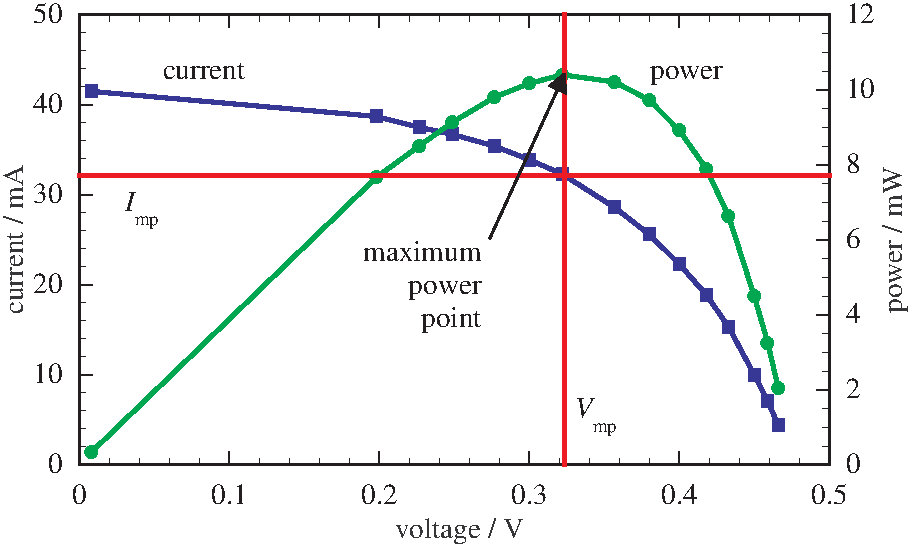
\includegraphics[scale=0.72]{solarcell}
\caption{Current and power as a function of voltage delivered by a single photovoltaic cell under illumination from a 150\,W metal halide floodlamp, showing the maximum power point.}
\label{solar cell fig}
\end{figure}

Figures and tables must have informative captions and be numbered as in Figure~\ref{solar cell fig}. Axes of graphs should have scales, titles and units, otherwise the plot is meaningless. All text must be legible, roughly the same size as the main text. Be warned that plots from Excel need extensive editing to bring them up to an acceptable standard. Oscilloscope screenshots can make good illustrations and are simple to capture on modern equipment.

Tables must have appropriate headings with units. Avoid lengthy tables: consider whether a graph would be clearer or the data would be better on a CD.

\subsection{References}

No project is done in isolation. A research project builds on the results of previous workers; a design-and-build project depends on the properties of the components available. You therefore draw on published documents during your project and must provide \emph{references} to these sources in your report. References are cited (a)~to give due credit to the originator and (b)~to guide a reader who wants more detailed information. You should give a reference wherever it is required for either of these purposes. Properly referenced material from many sources is a sign of a good project report. 
%This section explains how to present such references and how you will be penalised if you fail to do this. The mark for the report include an element for references to reflect their importance.

References must be cited with sequential numbers in square brackets where they are used in the text, not just listed at the end of the report. Typical usage is `Fitzmaurice and Hand \cite{gmf87} showed that\dots' or `The median is an appropriate estimator for this signal \cite{gmf87}'.

Avoid direct quotations from references in general; make it absolutely clear that the text is a quotation if this is unavoidable. An illustration, such as a diagram from a data sheet, is another type of quotation and must be referenced, typically in the figure caption. This is perfectly acceptable: do not waste time redrawing diagrams.

\subsubsection{Plagiarism}

If you copy from another person's work (project report, book, journal, web page or any other document) without acknowledging the source, you are guilty of \emph{plagiarism}. This is a disciplinary offence and the University has procedures for handling it. The failure to acknowledge a source is considered as plagiarism even if there was no deliberate intention to cheat. 

Avoid any risk of plagiarism by providing a reference for all sources that you use. Read the advice offered by the University Library and consult your supervisor if you are in any doubt. The University's \emph{Plagiarism Statement} is reproduced in Appendix \ref{plagiarism sect}.

\subsubsection{List of references}

All reports must have a section entitled `References' after the main text but before any appendices. This comprises a list of references, numbered to match the citations in the text. Each reference requires the following information and the cited references provide examples.
\begin{itemize}
\item
\textbf{Journal paper}: 
author(s), title of paper, name of journal, volume number, first page, last page and year \cite{gmf87}. 
Many journals now use article numbers instead of page numbers.
\item
\textbf{Book}: 
author(s), title, edition, publisher and year of publication \cite{jve05}.
Include the number of the chapter or page(s) if you refer to only a small part of the book.
\item
\textbf{Data sheet}: 
company, title, edition and date \cite{s08qg}. 
Application notes, technical reports and similar documents should be cited in the same way.
\item
\textbf{Web page}: 
author(s) or organisation, title, full URL and date of viewing \cite{mac09}. See below.
\end{itemize}
%The general rule is that 
The reader must be able to find the document without searching for further information.

\subsubsection{References from the Web}

The World Wide Web is a wonderful resource because it is so easy to search. It is therefore tempting to use web pages as references. \emph{Proceed with caution} because the accuracy of many web sites cannot be verified. This is particularly true for anonymous sites such as Wikipedia. Use them only as a starting point: good pages provide references to more authoritative sources.

Reports whose references are all or mainly from the web, especially from anonymous sites, will be penalised.


\section{Discussion}

The discussion is your opportunity to impress an expert with your depth of understanding. Don't worry so much about the non-expert reader -- she or he can skip to the Conclusions.

For a research project this section should provide a logical argument leading from the experimental observations to the final conclusions. Evaluate your results thoroughly and gain every possible piece of understanding from them. Compare the results in detail to other work in the field. This should be a \emph{critical} comparison so don't just say that your results are different from previous work; explain \emph{why}. Never say `The results were as expected' unless you have already described exactly what was expected!

The main purpose of the Discussion in a design-and-build project is to assess the performance of your product against the specification, showing its strengths and weaknesses.


\section{Conclusions}

Every report must have conclusions, built on the discussion. This section includes a summary of the main achievements of the work but is more than that. The noun `conclusion' can be defined as `a judgement or decision reached by reasoning' \cite{oupconc} so you should highlight what has been learnt as a result of your project. What is the big picture that the reader should take away? 

The Conclusions should include an assessment of the outcome against the original aims of the project. If you were unable to fulfil some aims, explain why. It is also useful to review the project plan (which should be included with the report). Did some tasks prove to be unexpectedly difficult, for instance?

\subsection{Suggestions for further work}

Almost every project leaves you with ideas for the future. Research typically answers some questions while opening new ones; by the end of a design-and-build project you may have thought of a superior approach. Examiners are impressed by intelligent suggestions for further work because they show that you really understand the project. It is often a sign of strength to identify the weak points and suggest solutions for them.


\clearpage % start appendices on a new page
\begin{thebibliography}{9}
%\addcontentsline{toc}{section}{References}
\bibitem{jve05}
Joan van Emden,
\textit{Writing for Engineers},
3rd Edition,
Palgrave Macmillan 
(2005).

\bibitem{mkm06}
Marun K. Mitra,
\textit{Effective Technical Communication: A Guide for Scientists and Engineers},
Oxford
(2006).

\bibitem{dfb09}
David F. Beer and David McMurrey,
\textit{A Guide to Writing as an Engineer},
3rd Edition,
Wiley
(2009).

\bibitem{tmy05}
Trevor M. Young,
\textit{Technical Writing A--Z: A Commonsense Guide to Engineering Reports and Theses},
American Society of Mechanical Engineers
(2005).

\bibitem{ronneberger2015unet}
O. Ronneberger, P. Fischer, and T. Brox,
\textit{U-Net: Convolutional networks for biomedical image segmentation},
in \textit{Proc. Medical Image Computing and Computer-Assisted Intervention (MICCAI)},
pp. 234--241,
2015.

\bibitem{isensee2021nnunet}
F. Isensee, P. F. Jaeger, S. A. A. Kohl, J. Petersen, and K. H. Maier-Hein,
\textit{nnU-Net: A self-configuring method for deep learning-based biomedical image segmentation},
Nature Methods,
\textbf{18},
203--211
(2021).

\bibitem{staal2004drive}
J. Staal, M. D. Abramoff, M. Niemeijer, M. A. Viergever, and B. van Ginneken,
\textit{Ridge-based vessel segmentation in color images of the retina},
IEEE Transactions on Medical Imaging,
\textbf{23}(4),
501--509
(2004).

\bibitem{hoover2000locating}
A. Hoover, V. Kouznetsova, and M. Goldbaum,
\textit{Locating blood vessels in retinal images by piecewise threshold probing of a matched filter response},
IEEE Transactions on Medical Imaging,
\textbf{19}(3),
203--210
(2000).

\bibitem{fraz2012ensemble}
M. M. Fraz, A. R. Rudnicka, C. G. Owen, and S. A. Barman,
\textit{An ensemble classification-based approach applied to retinal blood vessel segmentation},
IEEE Transactions on Biomedical Engineering,
\textbf{59}(9),
2538--2548
(2012).

\bibitem{budai2013robust}
A. Budai, R. Bock, A. Maier, J. Hornegger, and G. Michelson,
\textit{Robust vessel segmentation in fundus images},
International Journal of Biomedical Imaging,
\textbf{2013},
154860
(2013).

\bibitem{luo2025panet}
X. Luo, L. Peng, Z. Ke, J. Lin, and Z. Yu,
\textit{PA-Net: A hybrid architecture for retinal vessel segmentation},
Pattern Recognition,
\textbf{161},
111254
(2025).

\bibitem{lee2015dsn}
C.-Y. Lee, S. Xie, P. Gallagher, Z. Zhang, and Z. Tu,
\textit{Deeply-supervised nets},
in \textit{Proc. Artificial Intelligence and Statistics (AISTATS)},
pp. 562--570,
2015.

\bibitem{zhu2021deformabledetr}
X. Zhu, W. Su, L. Lu, B. Li, X. Wang, and J. Dai,
\textit{Deformable DETR: Deformable transformers for end-to-end object detection},
in \textit{Proc. International Conference on Learning Representations (ICLR)},
2021.

\bibitem{zhu2019dcnv2}
X. Zhu, H. Hu, S. Lin, and J. Dai,
\textit{Deformable ConvNets v2: More deformable, better results},
in \textit{Proc. IEEE/CVF Conference on Computer Vision and Pattern Recognition (CVPR)},
pp. 9308--9316,
2019.

\bibitem{hou2021coordatt}
Q. Hou, D. Zhou, and J. Feng,
\textit{Coordinate attention for efficient mobile network design},
in \textit{Proc. IEEE/CVF Conference on Computer Vision and Pattern Recognition (CVPR)},
pp. 13713--13722,
2021.

\bibitem{qi2023dsc}
J. Qi, Y. He, Y. Liu, and X. Xu,
\textit{Dynamic snake convolution based on topological geometric constraints for tubular structure segmentation},
in \textit{Proc. IEEE/CVF International Conference on Computer Vision (ICCV)},
pp. 6070--6079,
2023.

\bibitem{gmf87}
G M Fitzmaurice and D J Hand, 
\textit{A comparison of two average conditional error estimators}, 
Pattern Recognition Letters, 
\textbf{6}, 
221--228 
(1987).

\bibitem{s08qg}
Freescale Semiconductor,
\textit{Datasheet for MC9S08QG microcontroller},
revision 4
(2008).

\bibitem{mac09}
Morgan Advanced Ceramics, 
\textit{Advanced Ceramics: Silicon Nitride}, \texttt{www.morgantechnicalceramics.com} 
(viewed 2009 May 13).

\bibitem{oupconc}
Oxford University Press, 
\textit{AskOxford},
\texttt{www.askoxford.com/?view=uk}
(viewed 2009 May 13).

`Conclusion' is defined as (1)~an end or finish, (2)~the summing-up of an argument or text, (3)~a judgement or decision reached by reasoning or (4)~the settling of a treaty or agreement.
\end{thebibliography}

\clearpage % start appendices on a new page
\appendix

\section{Appendices}

Use appendices for supporting material which is relevant but of a detailed nature. In this way the flow of ideas in the body of the report is not interrupted. Appendices are usually lettered rather than numbered to distinguish them. Several uses for appendices have been suggested already but bear in mind that a CD may be more appropriate for large tables of results, long programs and data sheets or other background information. Appendices are not included in the word count because the assessors are not obliged to read them. Do not put vital points here!

Include your project plan and interim reports as appendices on paper.

\section{University's Plagiarism Statement}
\label{plagiarism sect}

The University's degrees and other academic awards are given in recognition of a student's personal achievement. All work submitted by students for assessment is accepted on the understanding that it is the student's own effort. 

Plagiarism is defined as the submission or presentation of work, in any form, which is not one's own, without acknowledgement of the sources. Plagiarism includes inappropriate collaboration with others. Special cases of plagiarism can arise from a student using his or her own previous work (termed auto-plagiarism or self-plagiarism). Autoplagiarism includes using work that has already been submitted for assessment at this University or for any other academic award.

The incorporation of material without formal and proper acknowledgement (even with no deliberate intent to cheat) can constitute plagiarism. Work may be considered to be plagiarised if it consists of: 
\begin{itemize}
\item
a direct quotation; 
\item
a close paraphrase; 
\item
an unacknowledged summary of a source; 
\item
direct copying or transcription.
\end{itemize}
With regard to essays, reports and dissertations, the rule is: if information or ideas are obtained from any source, that source must be acknowledged according to the appropriate convention in that discipline; and any direct quotation must be placed in quotation marks and the source cited immediately. Any failure to acknowledge adequately or to cite properly other sources in submitted work is plagiarism. Under examination conditions, material learnt by rote or close paraphrase will be expected to follow the usual rules of reference citation otherwise it will be considered as plagiarism. Departments should provide guidance on other appropriate use of references in examination conditions. 

Plagiarism is considered to be an act of fraudulence and an offence against University discipline. Alleged plagiarism, at whatever stage of a student's studies, whether before or after graduation, will be investigated and dealt with appropriately by the University.

The University reserves the right to use plagiarism detection systems, which may be externally based, in the interests of improving academic standards when assessing student work.

\end{document}
